\section{Benchmarks}

\hidenum
\begin{frame}[noframenumbering]
\frametitle{Contents}
 \tableofcontents[currentsection,hideallsubsections]
\end{frame}
\shownum

\subsection{Productivity Benchmark}

\begin{frame}[fragile]
\fontsize{8pt}{10}\selectfont
\begin{block}{Truncated SVD from Random Projections\footnotemark}
  \begin{minipage}{.55\textwidth}
    \begin{center}
      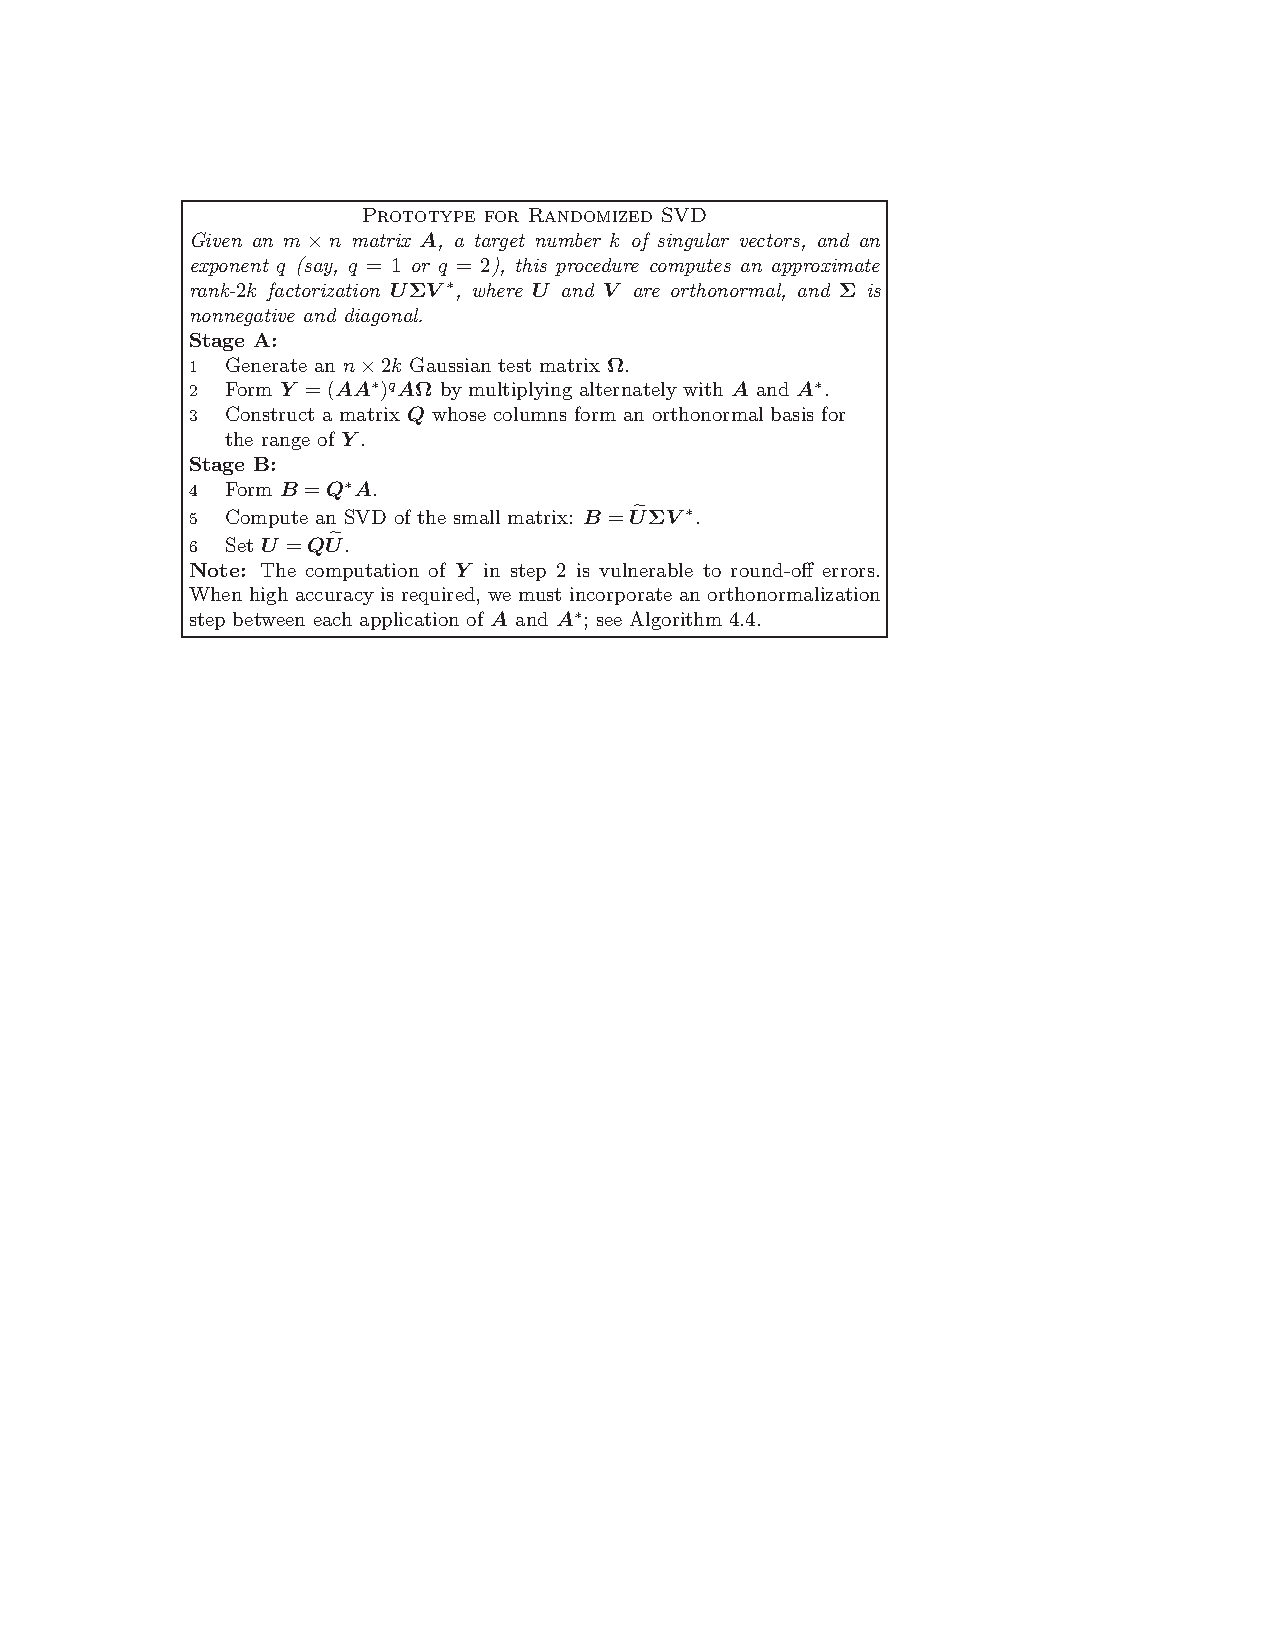
\includegraphics[width=.95\textwidth]{../common/pics/randSVDalg}
      \\
      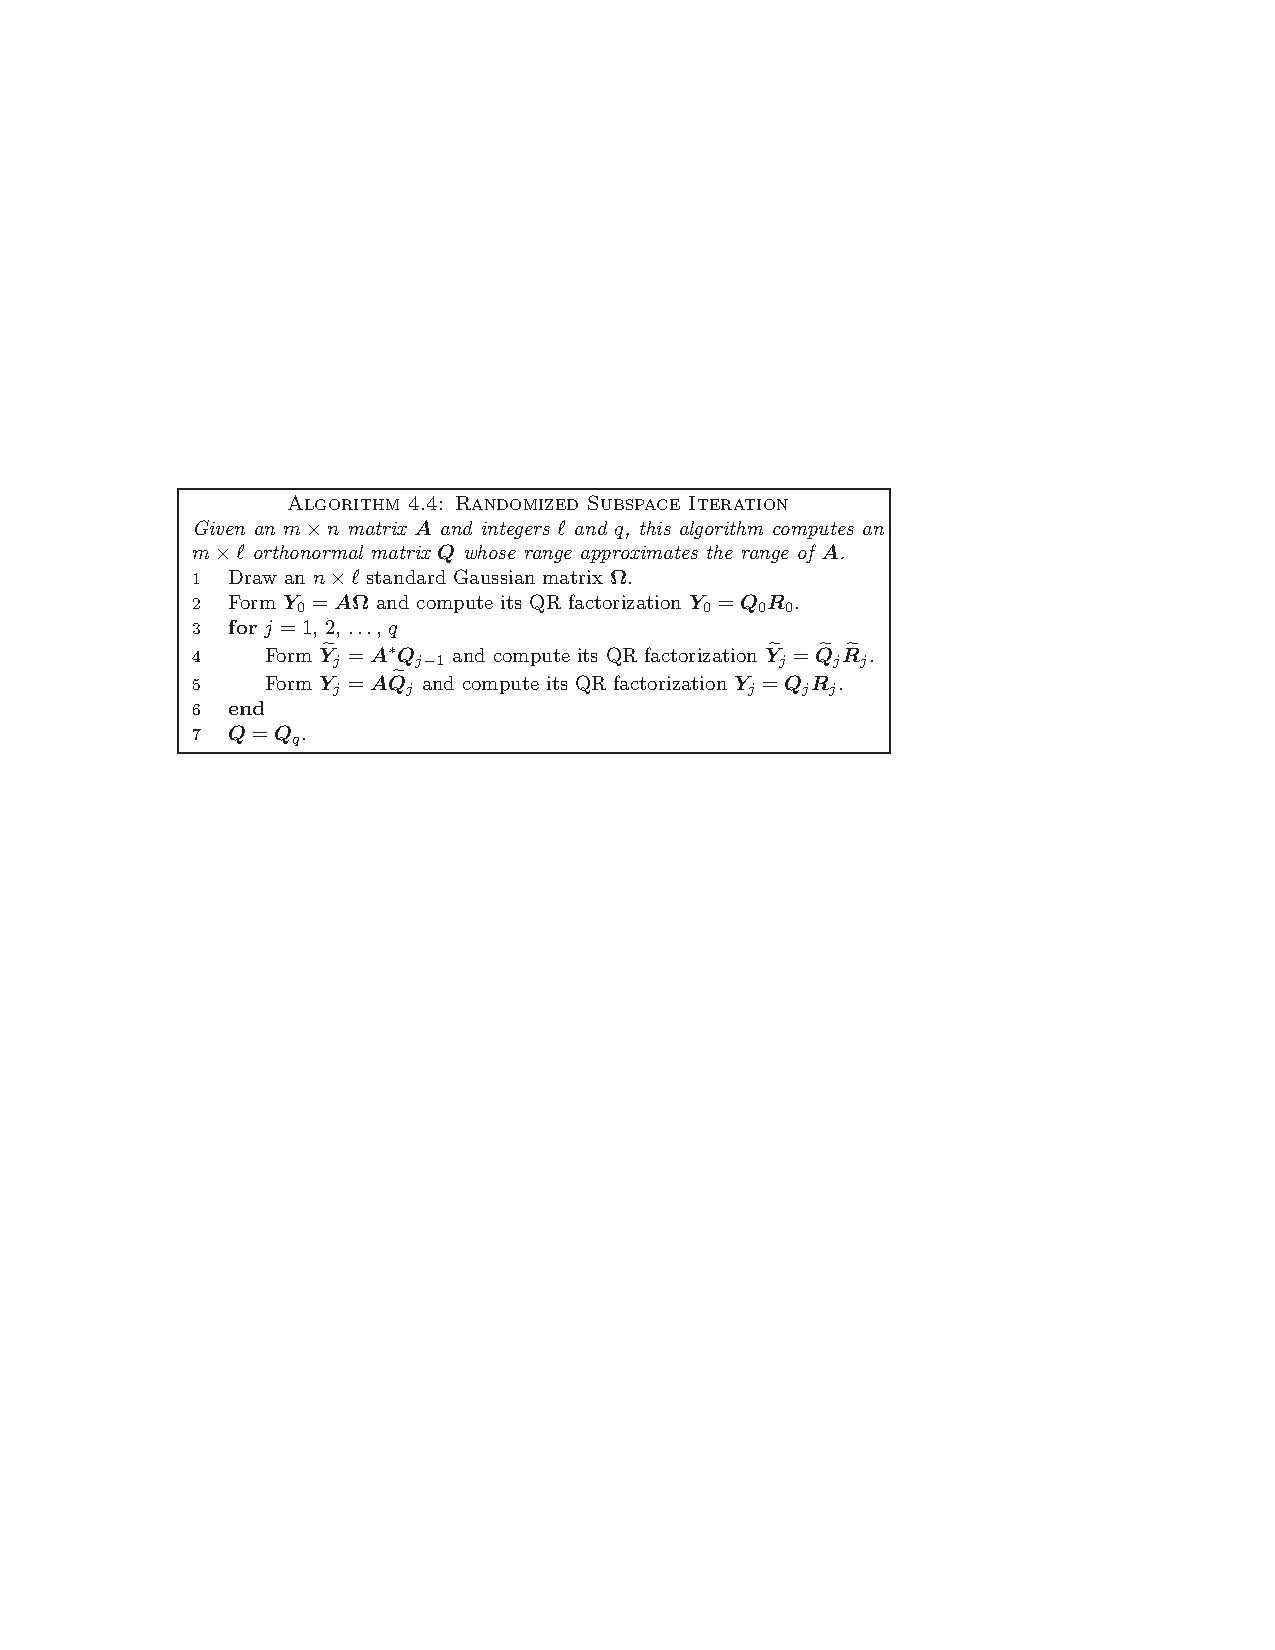
\includegraphics[width=.95\textwidth]{../common/pics/randSVDalg4_4}
    \end{center}
  \end{minipage}
%   \hspace{.01cm}
  \begin{minipage}{0.430\textwidth}
\begin{lstlisting}[title=Serial 
R,basicstyle=\tiny,backgroundcolor=\color{grayish} 
,numberstyle=\tiny\color{black},keywordstyle=\color{black},commentstyle=\color{ 
dkgreen},stringstyle=\color{black},escapeinside={(*@}{@*)}]
randSVD <- function(A, k, q=3)
  {
    ## Stage A
    Omega <- (*@ matrix(rnorm(n*2*k),@*) 
            (*@ nrow=n, ncol=2*k) @*)
    Y <- A %*% Omega
    Q <- qr.Q(qr(Y))
    At <- t(A)
    for(i in 1:q)
      {
        Y <- At %*% Q
        Q <- qr.Q(qr(Y))
        Y <- A %*% Q
        Q <- qr.Q(qr(Y))
      }
    
    ## Stage B
    B <- t(Q) %*% A
    U <- La.svd(B)$u
    U <- Q %*% U
    U[, 1:k]
  }
\end{lstlisting} %balance$
\end{minipage}
{\fontsize{6pt}{10}\selectfont $^1$Halko, Martinsson, 
  and Tropp, 2011. Finding structure with randomness: probabilistic algorithms 
  for constructing approximate matrix decompositions \emph{SIAM Review} \textbf{53} 
  217--288}
\end{block}
\end{frame}


\begin{frame}[fragile]
 \fontsize{8pt}{10}\selectfont
\begin{block}{Randomized SVD}
  \hfill
  \begin{minipage}{0.430\textwidth}
\begin{lstlisting}[title=Serial 
R,basicstyle=\tiny,backgroundcolor=\color{grayish} 
,numberstyle=\tiny\color{black},keywordstyle=\color{black},commentstyle=\color{ 
dkgreen},stringstyle=\color{black},escapeinside={(*@}{@*)}]
randSVD <- function(A, k, q=3)
  {
    ## Stage A
    Omega <- (*@ \textcolor{blue}{matrix(rnorm(n*2*k),} @*) 
         (*@ \textcolor{blue}{ nrow=n, ncol=2*k)} @*)
    Y <- A %*% Omega
    Q <- qr.Q(qr(Y))
    At <- t(A)
    for(i in 1:q)
      {
        Y <- At %*% Q
        Q <- qr.Q(qr(Y))
        Y <- A %*% Q
        Q <- qr.Q(qr(Y))
      }
    
    ## Stage B
    B <- t(Q) %*% A
    U <- La.svd(B)$u
    U <- Q %*% U
    U[, 1:k]
  }
\end{lstlisting} %balance$
  \end{minipage}
  \hfill
  \begin{minipage}{0.430\textwidth}
\begin{lstlisting}[title=Parallel pbdR,basicstyle=\tiny,backgroundcolor=\color{
grayish}, numberstyle=\tiny\color{black},keywordstyle=\color{black},
commentstyle=\color{dkgreen},stringstyle=\color{black},escapeinside={(*@}{@*)}]
randSVD <- function(A, k, q=3)
  {
    ## Stage A
    Omega <- (*@ \textcolor{blue}{ddmatrix("rnorm",} @*)
         (*@ \textcolor{blue}{nrow=n, ncol=2*k)} @*)
    Y <- A %*% Omega
    Q <- qr.Q(qr(Y))
    At <- t(A)      
    for(i in 1:q)
      {
        Y <- At %*% Q   
        Q <- qr.Q(qr(Y))
        Y <- A %*% Q    
        Q <- qr.Q(qr(Y))
      }
    
    ## Stage B
    B <- t(Q) %*% A     
    U <- La.svd(B)$u 
    U <- Q %*% U     
    U[, 1:k]
  }
\end{lstlisting}  % balancing $
  \end{minipage}
\hfill
\end{block}
\end{frame}

\begin{frame}
  \begin{block}{Randomized SVD}
    \begin{center}
      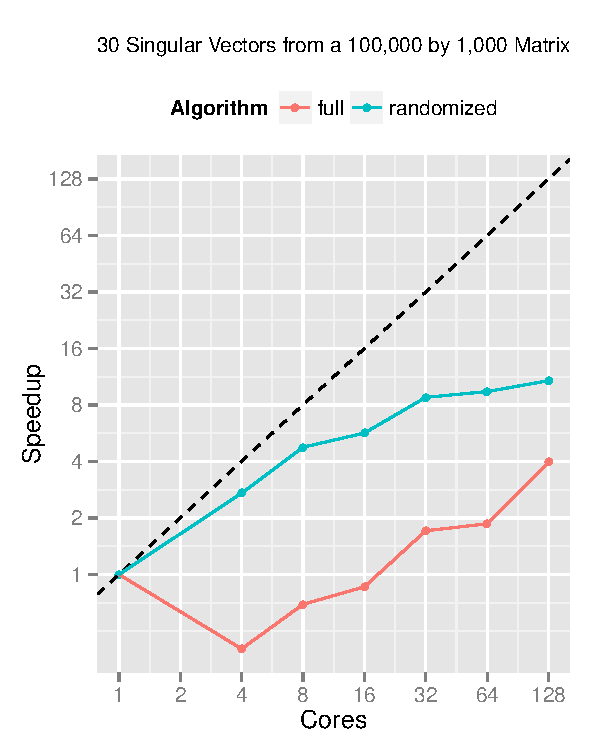
\includegraphics[width=.45\textwidth]{../common/pics/randSVDspeedup}
      \hfill
      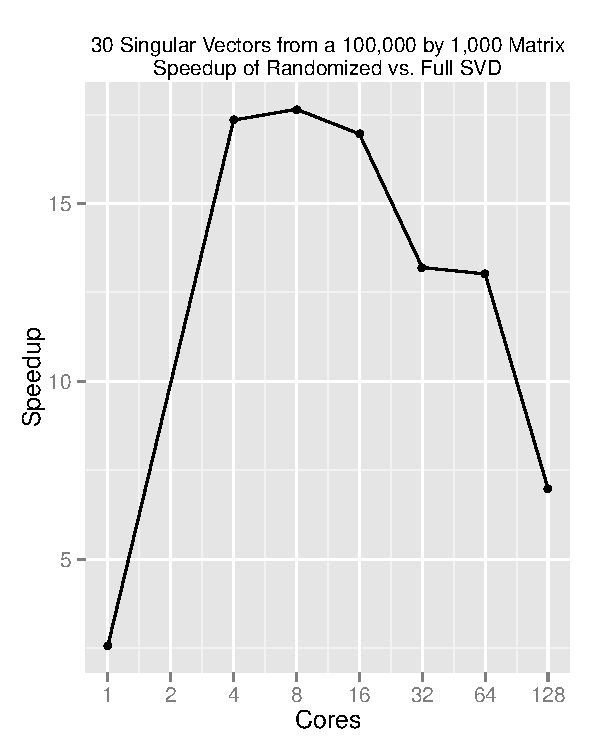
\includegraphics[width=.45\textwidth]{../common/pics/randSpeedupSVD}
    \end{center}
  \end{block}
\end{frame}

\subsection{Scalability Benchmarks}

\begin{frame}
  \begin{block}{Non-Optimal Choices Throughout}
    \begin{enumerate}[<+-|alert@+>]
      \item Only libre software used (no MKL, ACML, etc.).
      \item 1 core = 1 MPI process.
      \item No tuning for data layout.
    \end{enumerate}
  \end{block}
  \begin{block}{Benchmark Data}
    \begin{enumerate}[<+-|alert@+>]
      \item Random normal $N(100, 10000)$.
      \item Local problem size of $\approx 45.5 MB$.
      \item Three sets:  500, 1000, and 2000 columns.
      \item Several runs at different core sizes within each set.
    \end{enumerate}
  \end{block}
\end{frame}



% \subsection{Covariance}

\begin{frame}[fragile]
  \begin{block}{Covariance Code}
\begin{lstlisting}
x <- ddmatrix("rnorm", nrow=n, ncol=p, mean=mean, sd=sd)

cov.x <- cov(x)
\end{lstlisting}
  \end{block}
\end{frame}

\begin{frame}
  \begin{block}{\code{cov()}}
  \begin{center}
    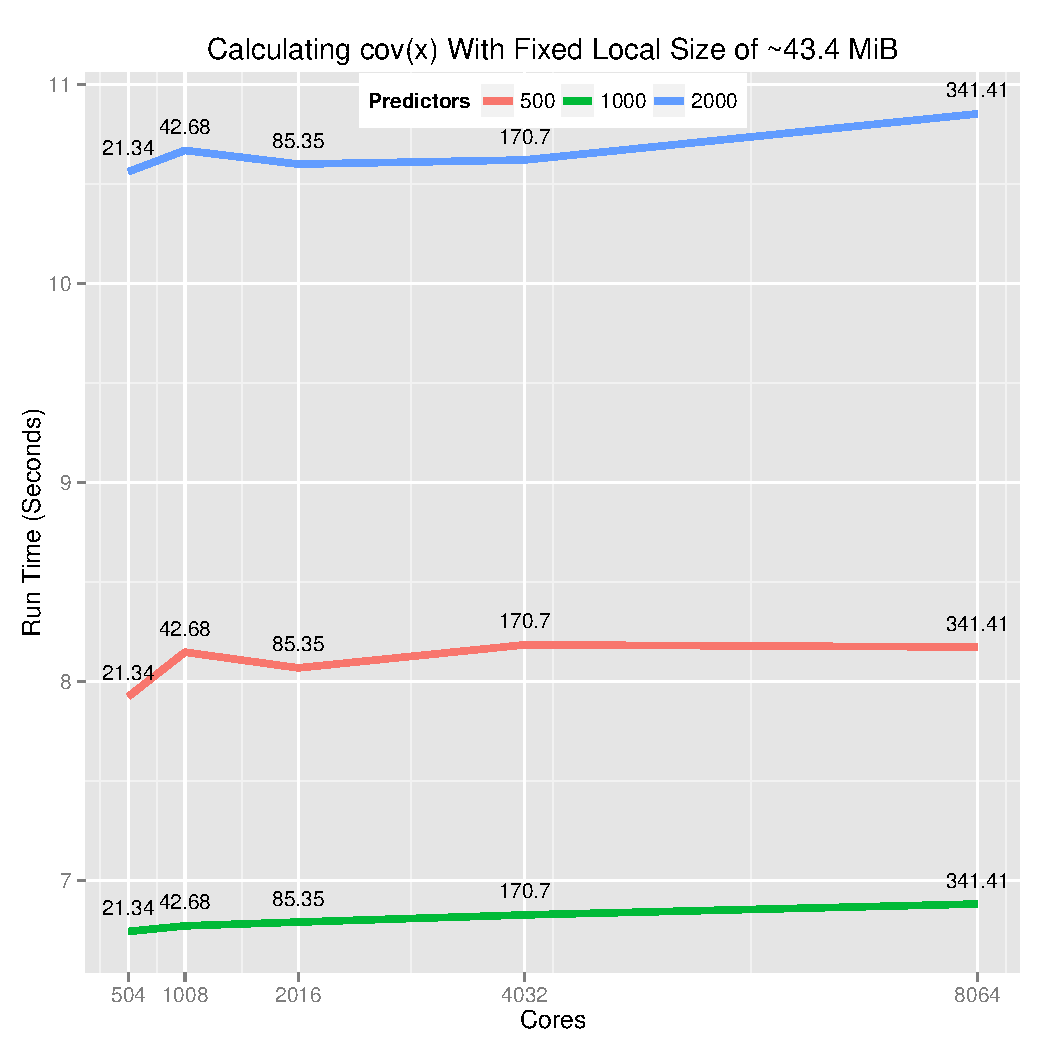
\includegraphics[height=.88\textheight]{../common/pics/cov}
  \end{center}
  \end{block}
\end{frame}



% \subsection{Linear Model Fitting}

\begin{frame}[fragile]
  \begin{block}{Linear Model Code}
\begin{lstlisting}
x <- ddmatrix("rnorm", nrow=n, ncol=p, mean=mean, sd=sd)
beta_true <- ddmatrix("runif", nrow=p, ncol=1)

y <- x %*% beta_true

beta_est <- lm.fit(x=x, y=y)$coefficients 
\end{lstlisting}
  \end{block}
\end{frame}

\begin{frame}
  \begin{block}{\code{Data Generation}}
  \begin{center}
    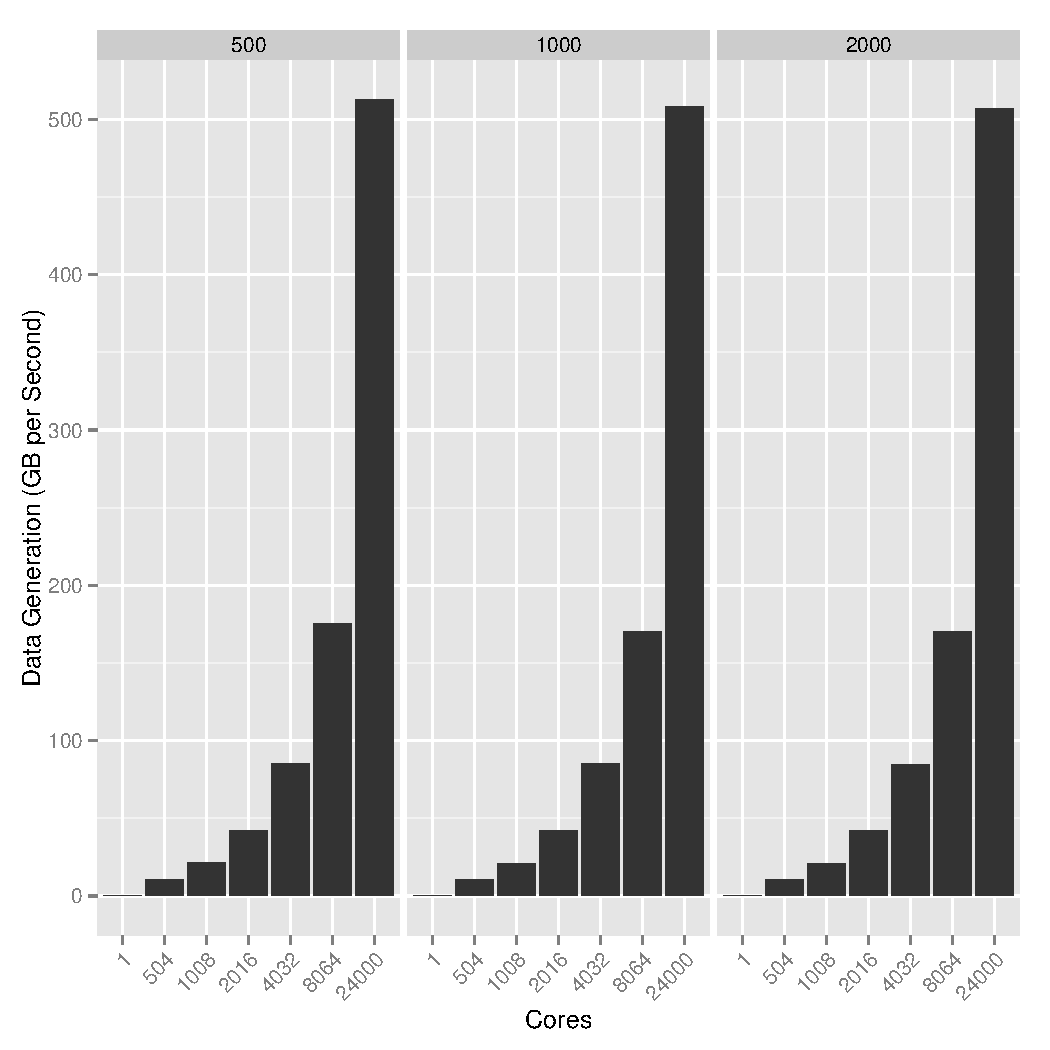
\includegraphics[height=.88\textheight]{../common/pics/datagen}
  \end{center}
  \end{block}
\end{frame}

% \begin{frame}
%   \begin{block}{\code{lm.fit()}}
%   \begin{center}
%     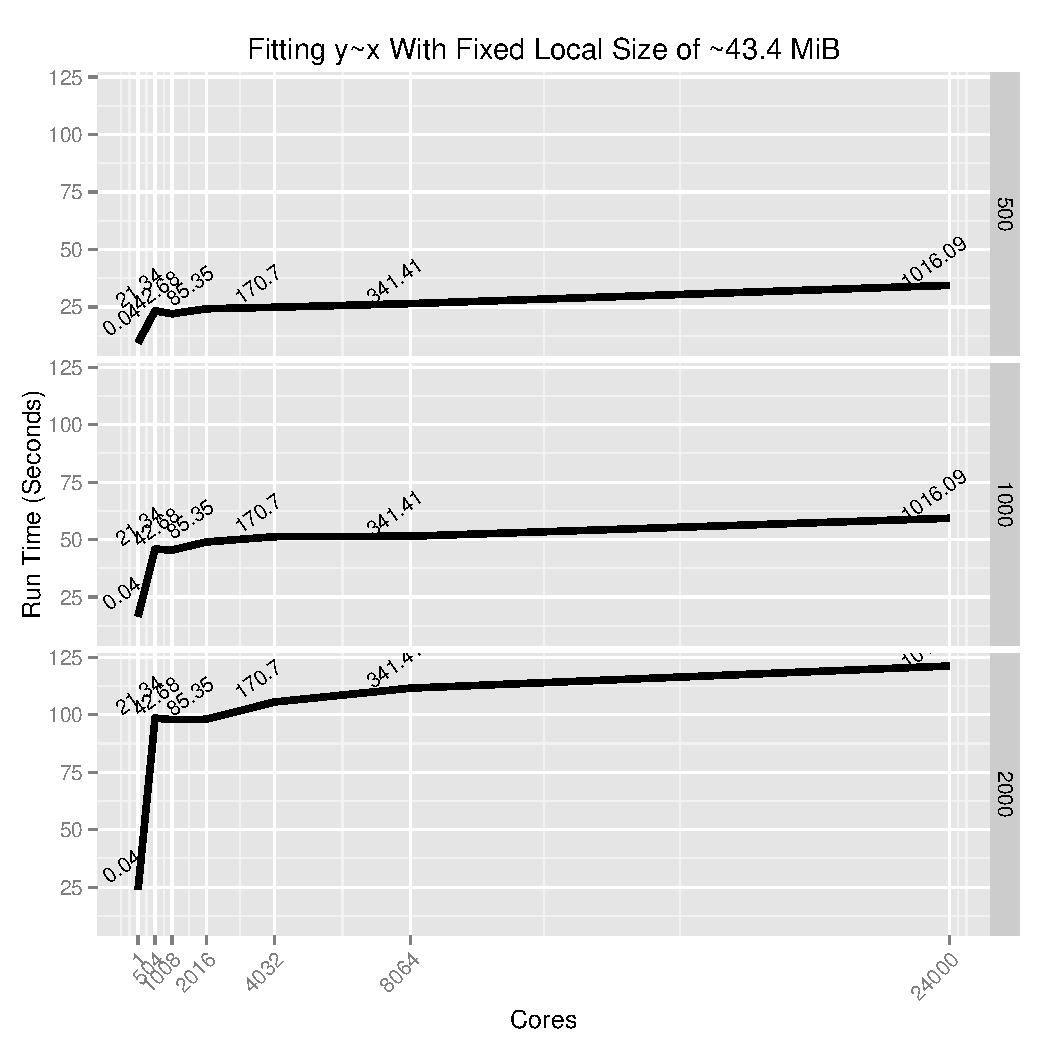
\includegraphics[height=.88\textheight]{../common/pics/lmfit1}
%   \end{center}
%   \end{block}
% \end{frame}

\begin{frame}
  \begin{block}{\code{lm.fit()}}
  \begin{center}
    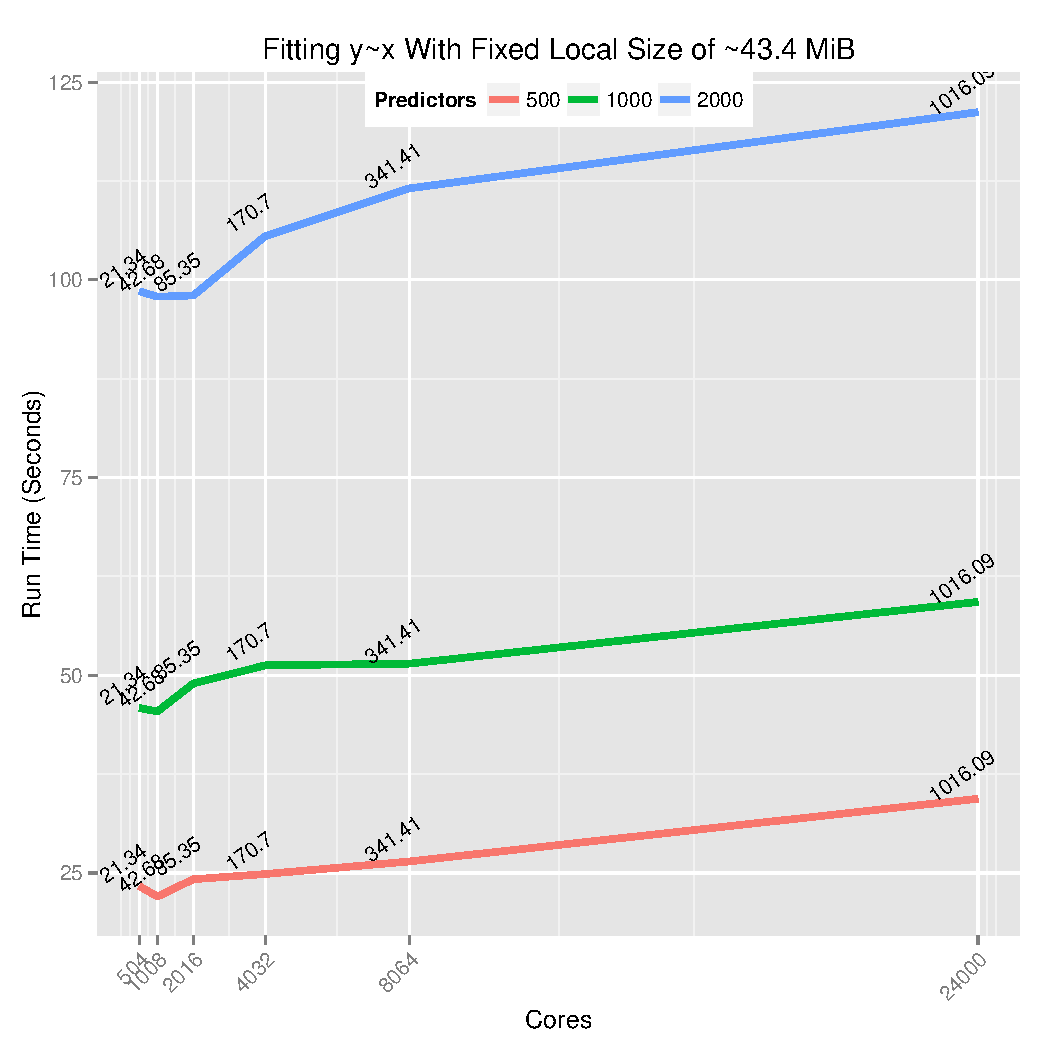
\includegraphics[height=.88\textheight]{../common/pics/lmfit2}
  \end{center}
  \end{block}
\end{frame}